\documentclass[aspectratio=169]{beamer}
\usetheme{Madrid}
\usecolortheme{default}

% Packages
\usepackage{graphicx}
\usepackage{listings}
\usepackage{xcolor}
\usepackage{tikz}
\usepackage{fontawesome5}

% Code styling
\lstset{
    language=PHP,
    basicstyle=\ttfamily\footnotesize,
    keywordstyle=\color{blue}\bfseries,
    commentstyle=\color{green!60!black},
    stringstyle=\color{red},
    numbers=left,
    numberstyle=\tiny\color{gray},
    stepnumber=1,
    numbersep=5pt,
    backgroundcolor=\color{gray!10},
    frame=single,
    breaklines=true,
    breakatwhitespace=true,
    tabsize=2,
    showspaces=false,
    showstringspaces=false,
    showtabs=false
}

% Title information
\title[Coffee Finder]{Coffee Finder Application}
\subtitle{Laravel Web Application Development Progress Report}
\author{[Your Name]}
\institute{University of the West of Scotland}
\date{\today}

\begin{document}

% Title slide
\begin{frame}
\titlepage
\end{frame}

% Table of Contents
\begin{frame}{Outline}
\tableofcontents
\end{frame}

% ============================================
% SECTION 1: PROJECT OVERVIEW
% ============================================
\section{Project Overview}

\begin{frame}{Project Overview}
\begin{columns}
\column{0.5\textwidth}
\textbf{Coffee Finder} is a web-based content management system designed to help users discover and share information about coffee shops.

\vspace{0.3cm}
\textbf{Key Features:}
\begin{itemize}
    \item CRUD Operations
    \item Image Upload with Metadata
    \item User Authentication \& Authorization
    \item Role-Based Access Control
    \item Responsive Bootstrap UI
\end{itemize}

\column{0.5\textwidth}
\begin{center}
% PLACEHOLDER: Screenshot of homepage
\fbox{\parbox{0.9\textwidth}{\centering
    \vspace{2cm}
    \textbf{[SCREENSHOT: Homepage]}\\
    \textit{Take screenshot of:}\\
    \texttt{http://localhost:8000/coffee-shops}\\
    \textit{or deployed URL}
    \vspace{2cm}
}}
\end{center}
\end{columns}
\end{frame}

\begin{frame}{Technology Stack}
\begin{center}
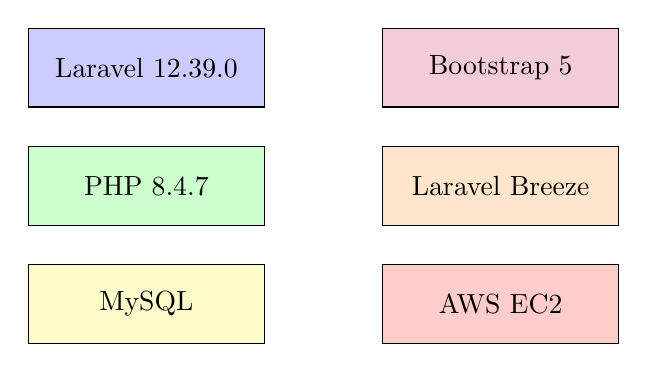
\begin{tikzpicture}[node distance=1.5cm]
    \node[draw, rectangle, fill=blue!20, minimum width=3cm, minimum height=1cm] (laravel) {Laravel 12.39.0};
    \node[draw, rectangle, fill=green!20, minimum width=3cm, minimum height=1cm, below of=laravel] (php) {PHP 8.4.7};
    \node[draw, rectangle, fill=yellow!20, minimum width=3cm, minimum height=1cm, below of=php] (mysql) {MySQL};
    \node[draw, rectangle, fill=purple!20, minimum width=3cm, minimum height=1cm, right of=laravel, xshift=3cm] (bootstrap) {Bootstrap 5};
    \node[draw, rectangle, fill=orange!20, minimum width=3cm, minimum height=1cm, below of=bootstrap] (breeze) {Laravel Breeze};
    \node[draw, rectangle, fill=red!20, minimum width=3cm, minimum height=1cm, below of=breeze] (aws) {AWS EC2};
\end{tikzpicture}
\end{center}
\end{frame}

% ============================================
% SECTION 2: DEVELOPMENT PROGRESS
% ============================================
\section{Development Progress}

\begin{frame}{MVC Architecture Implementation}
\begin{columns}
\column{0.5\textwidth}
\textbf{Models:}
\begin{itemize}
    \item \texttt{User} - Authentication
    \item \texttt{CoffeeShop} - Main entity
    \item \texttt{CoffeeShopImage} - Image metadata
\end{itemize}

\vspace{0.3cm}
\textbf{Controllers:}
\begin{itemize}
    \item \texttt{CoffeeShopController}
    \item \texttt{CoffeeShopImageController}
    \item \texttt{ProfileController}
\end{itemize}

\vspace{0.3cm}
\textbf{Views:}
\begin{itemize}
    \item Blade templates
    \item Bootstrap components
    \item Form validation
\end{itemize}

\column{0.5\textwidth}
\begin{lstlisting}[language=PHP, basicstyle=\tiny]
// app/Models/CoffeeShop.php
class CoffeeShop extends Model
{
    protected $fillable = [
        'name', 'description',
        'address', 'phone',
        'website', 'user_id'
    ];

    public function user()
    {
        return $this->belongsTo(User::class);
    }

    public function images()
    {
        return $this->hasMany(
            CoffeeShopImage::class
        );
    }
}
\end{lstlisting}
\end{columns}
\end{frame}

\begin{frame}{Database Schema}
\begin{center}
% PLACEHOLDER: Database diagram
\fbox{\parbox{0.9\textwidth}{\centering
    \vspace{2cm}
    \textbf{[SCREENSHOT: Database Schema]}\\
    \textit{Take screenshot of:}\\
    \texttt{phpMyAdmin} or \texttt{MySQL Workbench}\\
    \textit{showing tables: users, coffee\_shops, coffee\_shop\_images}
    \vspace{2cm}
}}
\end{center}
\end{frame}

\begin{frame}{Database Migrations}
\begin{columns}
\column{0.5\textwidth}
\begin{lstlisting}[language=PHP, basicstyle=\tiny]
// Migration: create_coffee_shops_table
Schema::create('coffee_shops', 
    function (Blueprint $table) {
        $table->id();
        $table->string('name');
        $table->text('description');
        $table->string('address');
        $table->string('phone')->nullable();
        $table->string('website')->nullable();
        $table->foreignId('user_id')
            ->constrained()
            ->onDelete('cascade');
        $table->timestamps();
    }
);
\end{lstlisting}

\column{0.5\textwidth}
\begin{lstlisting}[language=PHP, basicstyle=\tiny]
// Migration: create_coffee_shop_images_table
Schema::create('coffee_shop_images',
    function (Blueprint $table) {
        $table->id();
        $table->foreignId('coffee_shop_id')
            ->constrained()
            ->onDelete('cascade');
        $table->string('title');
        $table->text('description');
        $table->string('image_path');
        $table->timestamps();
    }
);
\end{lstlisting}
\end{columns}
\end{frame}

% ============================================
% SECTION 3: CHALLENGES AND SOLUTIONS
% ============================================
\section{Challenges \& Solutions}

\begin{frame}{Challenge 1: ViteManifestNotFoundException}
\begin{columns}
\column{0.5\textwidth}
\textbf{Problem:}
\begin{itemize}
    \item Application threw \texttt{ViteManifestNotFoundException}
    \item Laravel Breeze uses Vite by default
    \item Required Node.js and npm setup
    \item Complicated deployment process
\end{itemize}

\vspace{0.3cm}
\textbf{Solution:}
\begin{itemize}
    \item Replaced \texttt{@vite} directives
    \item Used Bootstrap CDN instead
    \item Simplified asset management
    \item No build process required
\end{itemize}

\column{0.5\textwidth}
\begin{lstlisting}[language=PHP, basicstyle=\tiny]
<!-- Before: layouts/app.blade.php -->
@vite(['resources/css/app.css',
       'resources/js/app.js'])

<!-- After: layouts/app.blade.php -->
<link href="https://cdn.jsdelivr.net/npm/
bootstrap@5.3.0/dist/css/bootstrap.min.css"
      rel="stylesheet">
<script src="https://cdn.jsdelivr.net/npm/
bootstrap@5.3.0/dist/js/bootstrap.bundle.min.js">
</script>
\end{lstlisting}
\end{columns}
\end{frame}

\begin{frame}{Challenge 1: Error Screenshot}
\begin{center}
% PLACEHOLDER: Error screenshot
\fbox{\parbox{0.9\textwidth}{\centering
    \vspace{2cm}
    \textbf{[SCREENSHOT: ViteManifestNotFoundException]}\\
    \textit{Take screenshot of:}\\
    Browser error page showing:\\
    \texttt{ViteManifestNotFoundException}\\
    \textit{If you don't have this, show the fixed version}
    \vspace{2cm}
}}
\end{center}
\end{frame}

\begin{frame}{Challenge 2: Route Order Conflict}
\begin{columns}
\column{0.5\textwidth}
\textbf{Problem:}
\begin{itemize}
    \item Accessing \texttt{/coffee-shops/create} returned 404
    \item Route was registered correctly
    \item Laravel matched wrong route
\end{itemize}

\vspace{0.3cm}
\textbf{Root Cause:}
\begin{itemize}
    \item Routes matched top-to-bottom
    \item \texttt{\{coffee\_shop\}} route matched first
    \item "create" treated as ID parameter
\end{itemize}

\column{0.5\textwidth}
\begin{lstlisting}[language=PHP, basicstyle=\tiny]
// WRONG ORDER:
Route::get('coffee-shops/{coffee_shop}',
    [CoffeeShopController::class, 'show']);

Route::get('coffee-shops/create',
    [CoffeeShopController::class, 'create']);

// CORRECT ORDER:
Route::get('coffee-shops/create',
    [CoffeeShopController::class, 'create']);

Route::get('coffee-shops/{coffee_shop}',
    [CoffeeShopController::class, 'show']);
\end{lstlisting}
\end{columns}
\end{frame}

\begin{frame}{Challenge 2: Error Screenshot}
\begin{center}
% PLACEHOLDER: 404 error screenshot
\fbox{\parbox{0.9\textwidth}{\centering
    \vspace{2cm}
    \textbf{[SCREENSHOT: 404 Error on /coffee-shops/create]}\\
    \textit{Take screenshot of:}\\
    Browser showing 404 error when accessing:\\
    \texttt{http://localhost:8000/coffee-shops/create}\\
    \textit{Or show the fixed working page}
    \vspace{2cm}
}}
\end{center}
\end{frame}

\begin{frame}{Challenge 3: Authorization Method Missing}
\begin{columns}
\column{0.5\textwidth}
\textbf{Problem:}
\begin{itemize}
    \item \texttt{Call to undefined method authorize()}
    \item Controller couldn't use authorization
    \item Base Controller was empty
\end{itemize}

\vspace{0.3cm}
\textbf{Solution:}
\begin{itemize}
    \item Added \texttt{AuthorizesRequests} trait
    \item Added \texttt{ValidatesRequests} trait
    \item Extended \texttt{BaseController}
\end{itemize}

\column{0.5\textwidth}
\begin{lstlisting}[language=PHP, basicstyle=\tiny]
// app/Http/Controllers/Controller.php
namespace App\Http\Controllers;

use Illuminate\Foundation\Auth\
    Access\AuthorizesRequests;
use Illuminate\Foundation\Validation\
    ValidatesRequests;
use Illuminate\Routing\Controller 
    as BaseController;

abstract class Controller 
    extends BaseController
{
    use AuthorizesRequests, 
        ValidatesRequests;
}
\end{lstlisting}
\end{columns}
\end{frame}

\begin{frame}{Challenge 3: Error Screenshot}
\begin{center}
% PLACEHOLDER: Authorization error
\fbox{\parbox{0.9\textwidth}{\centering
    \vspace{2cm}
    \textbf{[SCREENSHOT: Authorization Error]}\\
    \textit{Take screenshot of:}\\
    Browser error page showing:\\
    \texttt{Call to undefined method}\\
    \texttt{App\Http\Controllers\CoffeeShopImageController::authorize()}\\
    \textit{Or Laravel error page}
    \vspace{2cm}
}}
\end{center}
\end{frame}

% ============================================
% SECTION 4: CODE EXTRACTS
% ============================================
\section{Code Extracts \& Documentation}

\begin{frame}{CRUD Operations: Create}
\begin{columns}
\column{0.5\textwidth}
\begin{lstlisting}[language=PHP, basicstyle=\tiny]
// CoffeeShopController@store
public function store(Request $request)
{
    $validated = $request->validate([
        'name' => 'required|string|max:255',
        'description' => 'required|string',
        'address' => 'required|string',
        'phone' => 'nullable|string',
        'website' => 'nullable|url',
    ]);

    $coffeeShop = CoffeeShop::create([
        ...$validated,
        'user_id' => auth()->id(),
    ]);

    return redirect()
        ->route('coffee-shops.show', $coffeeShop)
        ->with('success', 'Coffee shop created!');
}
\end{lstlisting}

\column{0.5\textwidth}
% PLACEHOLDER: Create form screenshot
\fbox{\parbox{0.9\textwidth}{\centering
    \vspace{2cm}
    \textbf{[SCREENSHOT: Create Coffee Shop Form]}\\
    \textit{Take screenshot of:}\\
    \texttt{http://localhost:8000/coffee-shops/create}\\
    \textit{Showing the form with Bootstrap styling}
    \vspace{2cm}
}}
\end{columns}
\end{frame}

\begin{frame}{CRUD Operations: Update}
\begin{columns}
\column{0.5\textwidth}
\begin{lstlisting}[language=PHP, basicstyle=\tiny]
// CoffeeShopController@update
public function update(
    Request $request, 
    CoffeeShop $coffeeShop
) {
    $this->authorize('update', $coffeeShop);

    $validated = $request->validate([
        'name' => 'required|string|max:255',
        'description' => 'required|string',
        'address' => 'required|string',
        'phone' => 'nullable|string',
        'website' => 'nullable|url',
    ]);

    $coffeeShop->update($validated);

    return redirect()
        ->route('coffee-shops.show', $coffeeShop)
        ->with('success', 'Updated!');
}
\end{lstlisting}

\column{0.5\textwidth}
% PLACEHOLDER: Edit form screenshot
\fbox{\parbox{0.9\textwidth}{\centering
    \vspace{2cm}
    \textbf{[SCREENSHOT: Edit Coffee Shop Form]}\\
    \textit{Take screenshot of:}\\
    \texttt{http://localhost:8000/coffee-shops/1/edit}\\
    \textit{Showing form with existing data}
    \vspace{2cm}
}}
\end{columns}
\end{frame}

\begin{frame}{File Upload Implementation}
\begin{columns}
\column{0.5\textwidth}
\begin{lstlisting}[language=PHP, basicstyle=\tiny]
// CoffeeShopImageController@store
public function store(
    Request $request, 
    CoffeeShop $coffeeShop
) {
    $this->authorize('update', $coffeeShop);

    $validated = $request->validate([
        'title' => 'required|string|max:255',
        'description' => 'required|string',
        'image' => 'required|image|max:5120',
    ]);

    $path = $request->file('image')
        ->store('coffee-shop-images', 'public');

    $coffeeShop->images()->create([
        'title' => $validated['title'],
        'description' => $validated['description'],
        'image_path' => $path,
    ]);

    return redirect()
        ->route('coffee-shops.show', $coffeeShop)
        ->with('success', 'Image uploaded!');
}
\end{lstlisting}

\column{0.5\textwidth}
% PLACEHOLDER: Upload form screenshot
\fbox{\parbox{0.9\textwidth}{\centering
    \vspace{2cm}
    \textbf{[SCREENSHOT: Image Upload Form]}\\
    \textit{Take screenshot of:}\\
    \texttt{http://localhost:8000/coffee-shops/1/images/create}\\
    \textit{Showing upload form with preview}
    \vspace{2cm}
}}
\end{columns}
\end{frame}

\begin{frame}{Authorization Policy}
\begin{columns}
\column{0.5\textwidth}
\begin{lstlisting}[language=PHP, basicstyle=\tiny]
// app/Policies/CoffeeShopPolicy.php
class CoffeeShopPolicy
{
    public function update(User $user, 
                          CoffeeShop $coffeeShop)
    {
        return $user->id === 
               $coffeeShop->user_id 
            || $user->role === 'admin';
    }

    public function delete(User $user, 
                          CoffeeShop $coffeeShop)
    {
        return $user->id === 
               $coffeeShop->user_id 
            || $user->role === 'admin';
    }
}
\end{lstlisting}

\column{0.5\textwidth}
% PLACEHOLDER: Authorization test
\fbox{\parbox{0.9\textwidth}{\centering
    \vspace{2cm}
    \textbf{[SCREENSHOT: Authorization Test]}\\
    \textit{Take screenshot of:}\\
    User trying to edit another user's coffee shop\\
    \textit{Showing 403 Forbidden or no edit button}
    \vspace{2cm}
}}
\end{columns}
\end{frame}

\begin{frame}{Form Validation \& Repopulation}
\begin{columns}
\column{0.5\textwidth}
\begin{lstlisting}[language=PHP, basicstyle=\tiny]
<!-- resources/views/coffee-shops/create.blade.php -->
<form method="POST" 
      action="{{ route('coffee-shops.store') }}">
    @csrf
    
    <input type="text" 
           name="name" 
           value="{{ old('name') }}"
           class="form-control 
                  @error('name') is-invalid @enderror">
    
    @error('name')
        <div class="invalid-feedback">
            {{ $message }}
        </div>
    @enderror
    
    <button type="submit">Create</button>
</form>
\end{lstlisting}

\column{0.5\textwidth}
% PLACEHOLDER: Validation error
\fbox{\parbox{0.9\textwidth}{\centering
    \vspace{2cm}
    \textbf{[SCREENSHOT: Validation Errors]}\\
    \textit{Take screenshot of:}\\
    Form with validation errors displayed\\
    \textit{Showing red error messages and repopulated fields}
    \vspace{2cm}
}}
\end{columns}
\end{frame}

% ============================================
% SECTION 5: TECHNICAL UNDERSTANDING
% ============================================
\section{Technical Understanding}

\begin{frame}{MVC Architecture}
\begin{columns}
\column{0.5\textwidth}
\textbf{Model:}
\begin{itemize}
    \item Data structure
    \item Business logic
    \item Database relationships
\end{itemize}

\textbf{View:}
\begin{itemize}
    \item User interface
    \item Blade templates
    \item Presentation logic
\end{itemize}

\textbf{Controller:}
\begin{itemize}
    \item Request handling
    \item Validation
    \item Response generation
\end{itemize}

\column{0.5\textwidth}
% PLACEHOLDER: MVC diagram
\fbox{\parbox{0.9\textwidth}{\centering
    \vspace{2cm}
    \textbf{[DIAGRAM: MVC Flow]}\\
    \textit{Create or find diagram showing:}\\
    Request → Controller → Model → View → Response
    \vspace{2cm}
}}
\end{columns}
\end{frame}

\begin{frame}{Eloquent ORM Relationships}
\begin{columns}
\column{0.5\textwidth}
\begin{lstlisting}[language=PHP, basicstyle=\tiny]
// User Model
class User extends Authenticatable
{
    public function coffeeShops()
    {
        return $this->hasMany(
            CoffeeShop::class
        );
    }
}

// CoffeeShop Model
class CoffeeShop extends Model
{
    public function user()
    {
        return $this->belongsTo(User::class);
    }

    public function images()
    {
        return $this->hasMany(
            CoffeeShopImage::class
        );
    }
}
\end{lstlisting}

\column{0.5\textwidth}
% PLACEHOLDER: Relationship diagram
\fbox{\parbox{0.9\textwidth}{\centering
    \vspace{2cm}
    \textbf{[DIAGRAM: Database Relationships]}\\
    \textit{Create diagram showing:}\\
    User 1:N CoffeeShop 1:N CoffeeShopImage
    \vspace{2cm}
}}
\end{columns}
\end{frame}

\begin{frame}{HTTP Security: CSRF Protection}
\begin{columns}
\column{0.5\textwidth}
\textbf{CSRF Token:}
\begin{itemize}
    \item Prevents cross-site request forgery
    \item Laravel generates unique token
    \item Validated on POST requests
    \item Required in all forms
\end{itemize}

\vspace{0.3cm}
\textbf{Implementation:}
\begin{itemize}
    \item \texttt{@csrf} directive
    \item Automatic validation
    \item Token stored in session
\end{itemize}

\column{0.5\textwidth}
\begin{lstlisting}[language=PHP, basicstyle=\tiny]
<!-- Blade Template -->
<form method="POST" 
      action="{{ route('coffee-shops.store') }}">
    @csrf  <!-- CSRF Token -->
    
    <input type="text" name="name">
    <button type="submit">Submit</button>
</form>

<!-- Generated HTML -->
<form method="POST" 
      action="/coffee-shops">
    <input type="hidden" 
           name="_token" 
           value="abc123...">
    <input type="text" name="name">
    <button type="submit">Submit</button>
</form>
\end{lstlisting}
\end{columns}
\end{frame}

\begin{frame}{Role-Based Authorization}
\begin{columns}
\column{0.5\textwidth}
\textbf{User Roles:}
\begin{itemize}
    \item \texttt{admin} - Full access
    \item \texttt{user} - Own resources
    \item \texttt{guest} - Read only
\end{itemize}

\vspace{0.3cm}
\textbf{Implementation:}
\begin{itemize}
    \item Policy classes
    \item Middleware checks
    \item Blade directives
\end{itemize}

\column{0.5\textwidth}
\begin{lstlisting}[language=PHP, basicstyle=\tiny]
// Policy
public function update(User $user, 
                      CoffeeShop $coffeeShop)
{
    return $user->id === $coffeeShop->user_id
        || $user->role === 'admin';
}

// Controller
$this->authorize('update', $coffeeShop);

// Blade
@can('update', $coffeeShop)
    <a href="{{ route('coffee-shops.edit', $coffeeShop) }}">
        Edit
    </a>
@endcan
\end{lstlisting}
\end{columns}
\end{frame}

% ============================================
% SECTION 6: DEPLOYMENT
% ============================================
\section{Deployment \& Accessibility}

\begin{frame}{AWS EC2 Deployment}
\begin{columns}
\column{0.5\textwidth}
\textbf{Infrastructure:}
\begin{itemize}
    \item AWS EC2 Ubuntu Server
    \item Nginx Web Server
    \item PHP-FPM 8.4
    \item MySQL Database
    \item Let's Encrypt SSL
\end{itemize}

\vspace{0.3cm}
\textbf{Configuration:}
\begin{itemize}
    \item Environment variables
    \item Database connection
    \item Storage symlink
    \item File permissions
\end{itemize}

\column{0.5\textwidth}
% PLACEHOLDER: Deployment architecture
\fbox{\parbox{0.9\textwidth}{\centering
    \vspace{2cm}
    \textbf{[DIAGRAM: Deployment Architecture]}\\
    \textit{Create diagram showing:}\\
    Internet → Nginx → PHP-FPM → Laravel → MySQL
    \vspace{2cm}
}}
\end{columns}
\end{frame}

\begin{frame}{HTTPS Configuration}
\begin{columns}
\column{0.5\textwidth}
\begin{lstlisting}[basicstyle=\tiny]
# Nginx SSL Configuration
server {
    listen 443 ssl http2;
    server_name your-domain.duckdns.org;
    
    ssl_certificate 
        /etc/letsencrypt/live/your-domain.duckdns.org/fullchain.pem;
    ssl_certificate_key 
        /etc/letsencrypt/live/your-domain.duckdns.org/privkey.pem;
    
    root /var/www/coffee-finder/public;
    index index.php;
    
    location / {
        try_files $uri $uri/ /index.php?$query_string;
    }
    
    location ~ \.php$ {
        fastcgi_pass unix:/var/run/php/php8.4-fpm.sock;
        fastcgi_param SCRIPT_FILENAME 
            $realpath_root$fastcgi_script_name;
        include fastcgi_params;
    }
}
\end{lstlisting}

\column{0.5\textwidth}
% PLACEHOLDER: HTTPS browser
\fbox{\parbox{0.9\textwidth}{\centering
    \vspace{2cm}
    \textbf{[SCREENSHOT: HTTPS in Browser]}\\
    \textit{Take screenshot of:}\\
    Browser showing HTTPS lock icon\\
    \texttt{https://your-domain.duckdns.org}\\
    \textit{Address bar with green lock}
    \vspace{2cm}
}}
\end{columns}
\end{frame}

\begin{frame}{Public URL \& GitHub}
\begin{columns}
\column{0.5\textwidth}
\textbf{Public URL:}
\begin{itemize}
    \item \texttt{https://your-domain.duckdns.org}
    \item Accessible from anywhere
    \item HTTPS enabled
    \item SSL certificate valid
\end{itemize}

\vspace{0.3cm}
\textbf{GitHub Repository:}
\begin{itemize}
    \item Source code available
    \item Version control
    \item Commit history
    \item README documentation
\end{itemize}

\column{0.5\textwidth}
% PLACEHOLDER: GitHub repo
\fbox{\parbox{0.9\textwidth}{\centering
    \vspace{2cm}
    \textbf{[SCREENSHOT: GitHub Repository]}\\
    \textit{Take screenshot of:}\\
    GitHub repository page\\
    \textit{Showing repository structure and README}
    \vspace{2cm}
}}
\end{columns}
\end{frame}

% ============================================
% SECTION 7: LESSONS LEARNED
% ============================================
\section{Lessons Learned \& Conclusions}

\begin{frame}{Key Learnings}
\begin{columns}
\column{0.5\textwidth}
\textbf{Technical Skills:}
\begin{itemize}
    \item Laravel MVC architecture
    \item Eloquent ORM relationships
    \item Route organization
    \item Authorization policies
    \item File upload handling
\end{itemize}

\vspace{0.3cm}
\textbf{Problem Solving:}
\begin{itemize}
    \item Debugging techniques
    \item Error analysis
    \item Documentation reading
    \item Community resources
\end{itemize}

\column{0.5\textwidth}
\textbf{Best Practices:}
\begin{itemize}
    \item Route ordering matters
    \item Always validate input
    \item Use authorization policies
    \item Test thoroughly
    \item Document code
\end{itemize}

\vspace{0.3cm}
\textbf{Future Improvements:}
\begin{itemize}
    \item Search functionality
    \item Rating system
    \item Comments feature
    \item API development
\end{itemize}
\end{columns}
\end{frame}

\begin{frame}{Conclusion}
\begin{center}
\Large
\textbf{Coffee Finder Application}

\vspace{0.5cm}
Successfully developed and deployed a full-stack Laravel web application with:
\begin{itemize}
    \item Complete CRUD functionality
    \item Secure authentication \& authorization
    \item File upload with validation
    \item Responsive Bootstrap UI
    \item Public HTTPS deployment
\end{itemize}

\vspace{0.5cm}
\textbf{Public URL:} \texttt{https://your-domain.duckdns.org}

\vspace{0.5cm}
\textbf{GitHub:} \texttt{github.com/yourusername/coffee-finder}
\end{center}
\end{frame}

% Thank you slide
\begin{frame}
\begin{center}
\Huge Thank You!

\vspace{1cm}
\Large Questions?
\end{center}
\end{frame}

\end{document}

